\chapter{Systemkrav}
\label{Systemkrav}
%
I dette kapitel opstilles en generel produktbeskrivelse med specifikke systemkrav. Produktet beskrives først generelt ved hjælp af Use Cases og modultegninger. På baggrund af den generelle produktbeskrivelse formuleres en række specifikke systemkrav. De endelige krav vil til sidst opsummeres i prioriteret rækkefølge. 

\section{Generel Produktbeskrivelse}
\label{Generel_Produktbeskrivelse}
%
Målet for projektet er at udarbejde et elektronisk analogt produkt, som kan kompensere for menneskets frekvensafhængige perception af lydtryksniveauer. Produktet skal automatisk kunne filtrere et analogt lydsignal i relation til \textit{Normal Equal-Loudness-Level Contours} fremsat i \textcite{STD:ISO226}, på baggrund af lydtryksniveauet.\\
Selve filtreringen skal udelukkende foregå analogt for, at undgå at signalet forringes. Der skal derfor konstrueres en række analoge filtre, som kan forstærke eller dæmpe de lave frekvenser. Da filtreringen skal foregå automatisk på baggrund af lydtryksniveauet, er det nødvendigt at designe et system, som kan styre signalets vej igennem filtrende. Styresystemet skal derfor kunne detektere det aktuelle lydtryksniveau, samt referencespændingen, som angiver ved hvilket lydtryksniveau, et stykke musik er masterede ved, for derefter at kunne tilvælge eller fravælge de enkelte analoge filtre. Det aktuelle lydtryksniveau og referencespænding indstilles af den, der anvender produktet. Det skal derfor, ved hjælp af brugergrænsefladen, være muligt at ændre det aktuelle lydtryksniveau, ligesom det skal være muligt at ændre referencespænding. Det skal derudover være muligt at fravælge alle filtre på en gang, via en bypass-funktion. Bypass-funktionen skal kunne tilgås via brugergrænsefladen, samt sørge for at styresystemet leder signalet uden om filtrene.
   
\subsection{Use Cases} 
\label{UseCases}
%
Følgende afsnit fokuserer på de funktionelle krav produktet skal opfylde. Produktets funktioner beskrives ved hjælp af Use Cases, hvor grænseflader mellem aktører og funktioner vil fremgå. Den generelle produktbeskrivelse lægger op til uddybelse af produktets funktionelle krav, samt en opdelingen af de aktører, som indgår i processen.\\
Brugeren af produktet skal have mulighed for at ændre den aktuelle volumen, ændre referencespændingen samt bypasse samtlige filtre. Funktionerne; "Ændr volumen", "Ændr reference" og "Bypass" er derfor essentielle at implementere for at få produktet fungere optimalt. For at brugeren i sidste ende kan tilgå funktionerne er det nødvendigt at kende de interne og eksterne aktører, som er involveret i processerne. Som nævnt i \fullref{Generel_Produktbeskrivelse} er målet for projektet at fremstille et antal filtre, som ved hjælp af et styresystem kan til- eller fravælges, på baggrund af brugerens interaktion med brugergrænsefladen. De interne aktører; "Filtre", "Styresystem" og "Brugergrænseflade", symboliserer hvor der foregår en interaktion mellem produktets forskellige funktioner og specifikke moduler. Brugeren selv defineres som en ekstern aktør ligesom effektforstærkeren og højtaleren, der i sidste ende forstærker og afspiller signalet, også fremgår som eksterne aktører. Det sker for at simplificere Use Case diagrammet til kun at omfatte systemet selv. Use Case diagrammet på \autoref{fig:UseCaseDiagram} fokuserer derfor på de interne aktører, som gør funktionerne tilgængelige via grænsefladerne mellem funktion og aktør.       
%
\begin{figure}[H]
	\centering
	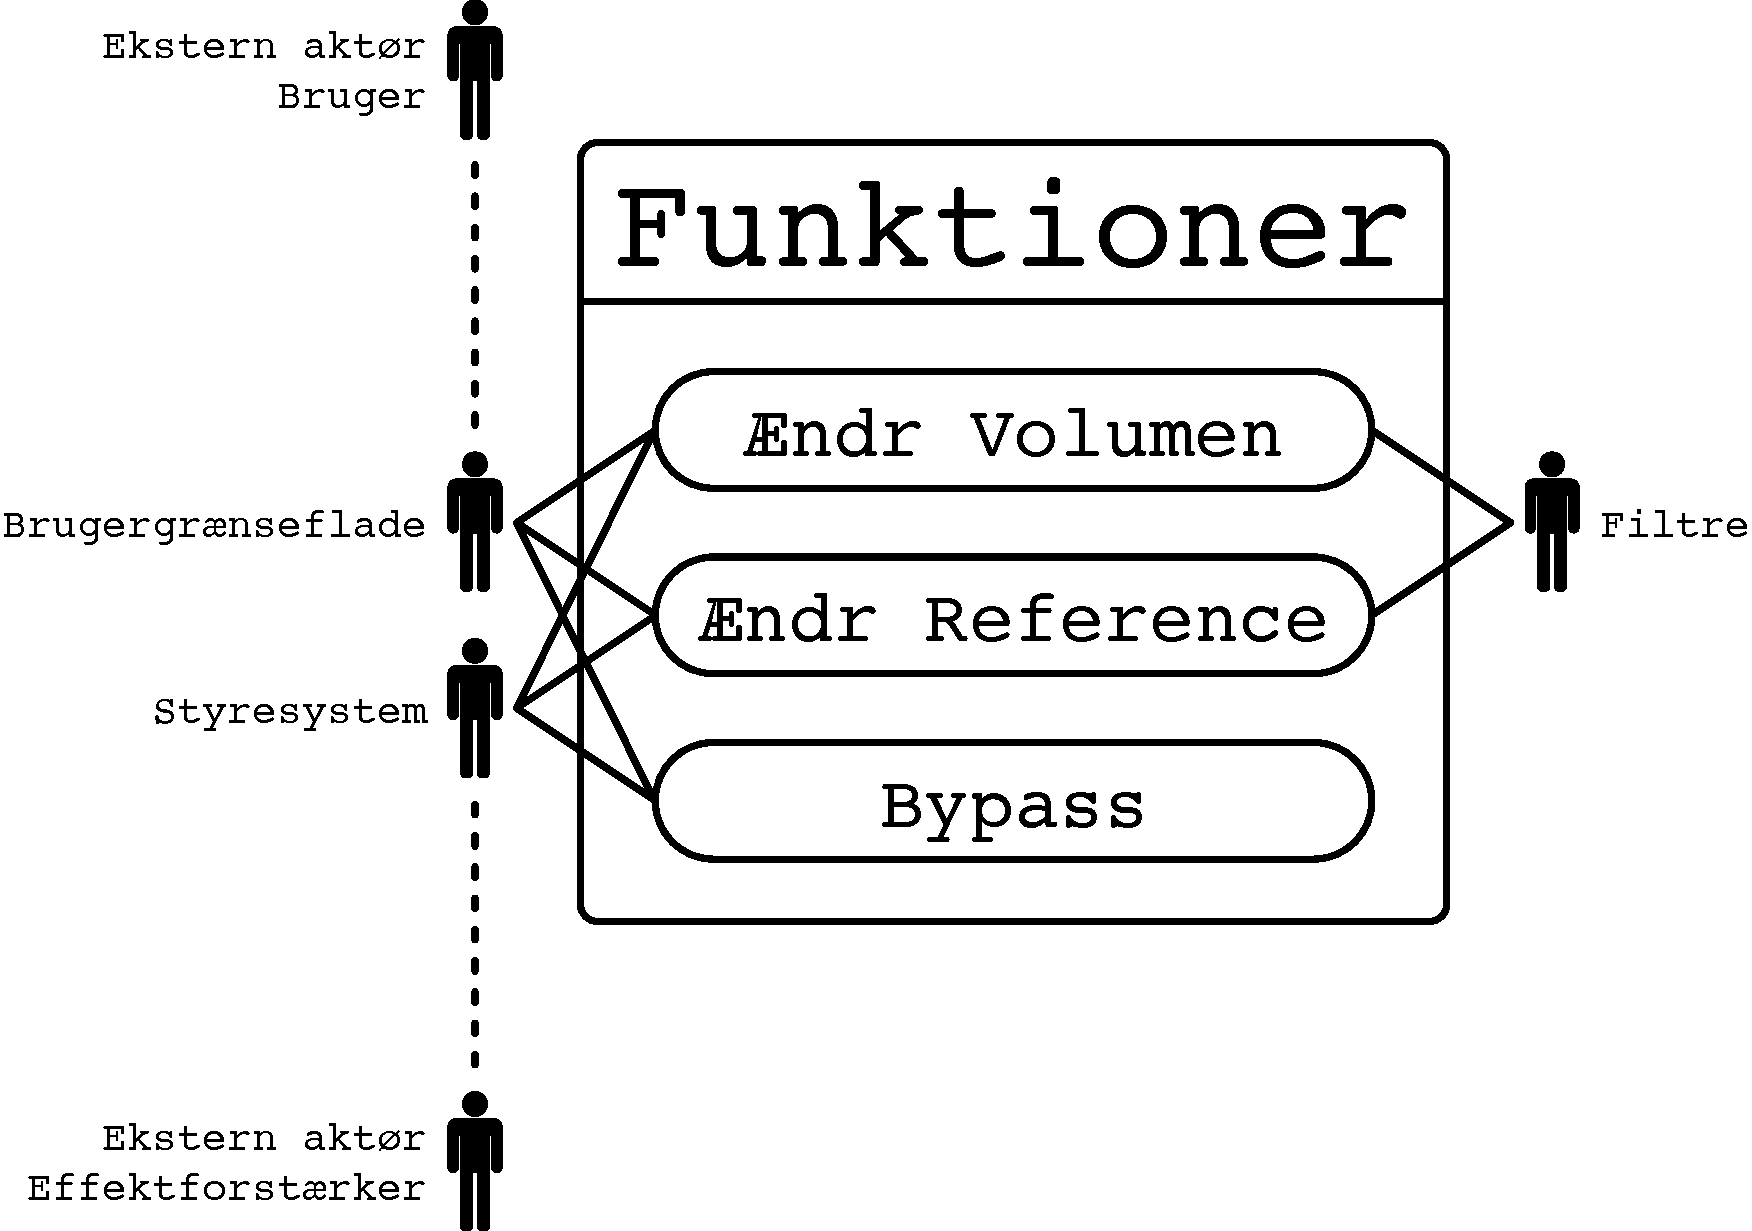
\includegraphics[resolution=300,scale=\circuitSize]{UseCaseDiagram}
	\caption{Use Case diagram for det samlede system. De tre Use Cases er forbundet til deres respektive aktører. Mellem Use Case og aktører findes grænsefladen, som er udtryk for hvilke aktører der kommunikerer med hinanden.}
	\label{fig:UseCaseDiagram}
\end{figure}
\noindent   

\subsubsection{Ændr volumen} 
\label{AendreVolumen}       
%
Brugeren interagerer med brugergrænsefladen for at ændre volumen, og dermed lydtryksniveauet for hvor musikken afspilles. Brugergrænsefladen signalerer via grænsefladen til styresystemet at der er sket en volumenændring. Styresystemet reagerer på ændringen og vælger via grænsefladen til filtrene, hvilke filtre der skal til- eller fravælges. Styresystemet signalerer via grænsefladen til brugergrænsefladen hvilke filtre der er til- eller fravalgt. 

\subsubsection{Ændr reference} 
\label{AendreReference}
%
Brugeren interagerer med brugergrænsefladen for at ændre referencevolumen. Brugergrænsefladen signalerer via grænsefladen til styresystemet at der er sket en ændring i referencevolumen. Styresystemet reagerer på ændringen og vælger via grænsefladen til filtrene, hvilke filtre der skal til- eller fravælges. Styresystemet signalerer via grænsefladen til brugergrænsefladen hvilke filtre der er til- eller fravalgt.

\subsubsection{Bypass}
\label{Bypass}
%
Brugeren interagerer med brugergrænsefladen for enten at aktivere eller deaktivere bypass-funktionen. Brugergrænsefladen signalerer via grænsefladen til styresystemet at der er sket en ændring i forhold til bypass. Styresystemet reagerer på ændringen og vælger via grænsefladen til filtrene om filtre skal til- eller fravælges. Styresystemet signalerer via grænsefladen til brugergrænsefladen om filtre er til- eller fravalgt. 
\blankline 
Ud fra Use Case diagrammet, repræsenteret på \autoref{fig:UseCaseDiagram}, og beskrivelserne af de enkelte funktioner, opsummeres kommunikationskravene mellem de enkelte aktører:
\blankline
\begin{itemize}
  \item Der er kommunikation mellem brugergrænseflade og styresystem.
  \item Der er kommunikation mellem styresystem og filtre.
  \item Der er ikke kommunikation mellem brugergrænseflade og filtre. Alt kommunikation herimellem foregår via styresystemet.
\end{itemize}
   
%  
\subsection{Moduloversigt} 
\label{Moduloversigt}
%
Følgende afsnit vil, ved hjælp af en moduloversigt, give et indblik i hvilke moduler de enkelte aktører består af. Moduloversigten er en overordnet skitse af det samlede system og skal virke til at konkretisere hvilke grænseflader der findes mellem de enkelte moduler i hver aktør. Moduloversigten er derfor delt op i tre grupper, så det tydeligt fremgår hvilken aktør modulerne tilhører, hvilket fremgår af \autoref{fig:ModulOversigt}. 
%
\begin{figure}[H]
	\centering
	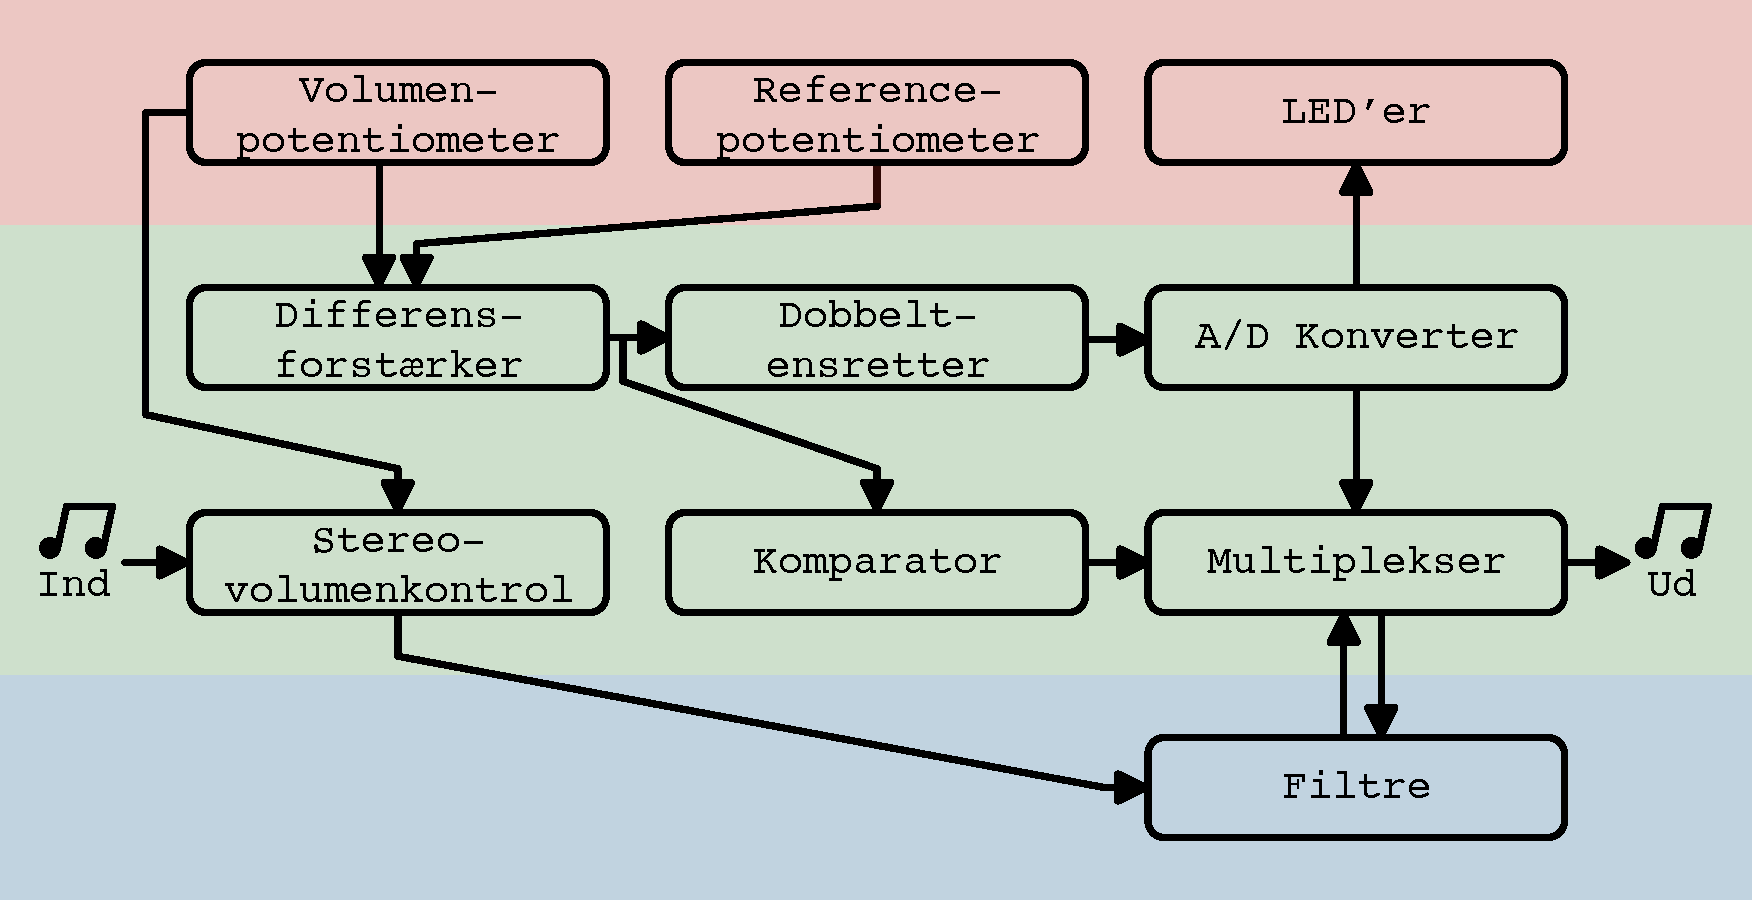
\includegraphics[resolution=300,scale=0.5]{ModulOversigt.pdf}
	\caption{Moduloversigt delt op i tre grupper, en for hver aktør: \textcolor{xRed}{Brugergrænseflade}, \textcolor{xGreen}{Styresystem} og \textcolor{xBlue}{Filtre}}
	\label{fig:ModulOversigt}
\end{figure}
\noindent
%
\subsubsection{Filtre}
\label{SystemkravFiltre}
%
Signalet, der skal behandles af filtrene, skal komme fra styresystemet, nærmere bestemt fra en stereovolumenkontrol. Signalet ledes både igennem og udenom de enkelte forstærkende og dæmpende filtre. Det sker for senere at gøre det muligt at vælge om det enkelte filter skal til- eller fravælges. Skal det enkelte filter ikke anvendes er det derved muligt at lede det ufiltrerede signal videre i systemet. Om de enkelte filtre skal tages i brug eller ej vælges af styresystemet, nærmere bestemt af en multiplekser. Multiplekseren virker som en kontaktfunktion der enten kan vælge at sende signalet fra et enkelt filter videre, eller sende det ufiltrerede signal videre. Signalet vælges og sendes igennem multiplekseren for derefter at ledes tilbage til filtrene. Igen ledes signalet både igennem og udenom det næste filter, hvorfra det er muligt at vælge om filteret skal tages i brug eller ej. Multiplekserens kontaktfunktion kan igen vælge om signalet, der sendes videre, skal filtreres eller ej. Denne proces fortsætter til signalet enten har været igennem eller forbi samtlige filtre.             
%
\subsubsection{Styresystem}
\label{SystemkravStyresystem}
Multiplekseren, som leder signalet igennem filtrene, styres ved hjælp af et digitalt binært signal fra A/D konverteren. Det er på den måde muligt at bestemme hvilke kontakter i multiplekseren, der skal være forbindelse imellem. Forbindelsen mellem kontakterne er afgørende for om signalet der sendes igennem filtreres. Yderligere modtager multiplekseren et input fra komparatoren. Komparatoren fortæller multiplekseren, efter signalet har passeret samtlige filtre, om signalet der sendes videre til effektforstærkeren skal være det forstærkede eller dæmpede signal.\par
Komparatorens output til multiplekseren afgøres af differensforstærkeren. Hvis differensforstærkerens output er positivt, fortæller komparatoren til multiplekseren at det dæmpede signal skal sendes videre. Hvis differensforstærkerens output i stedet er negativt, fortæller komparatoren til multiplekseren at det forstærkede signal skal sendes videre.\par
Dobbeltensretteren sørger for at alle negative outputs fra differensforstærkeren gøres positive, inden de sendes videre til A/D konverteren, da A/D konverteren kun arbejder med positive spændinger. Det er derfor komparatorens opgave at tjekke om signalet er negativt eller positivt før det sendes igennem dobbeltensretteren. Både A/D konverteren og komparatoren sender besked videre til brugergrænsefladen så en visuel repræsentation af de aktuelle filtre fremgår på et display med LED'er. Differensforstærkerens positive eller negative output afgøres af differencen mellem  volumen- og referencepotentiometeret. 
%
\subsubsection{Brugergrænseflade}
\label{SystemkravBrugergraenseflade}
%
 Volumenpotentiometeret bestemmer hvor meget signal stereovolumenkontrollen lukker igennem, og dermed hvor kraftigt signalet, der løber igennem filtrene bliver. Volumenpotentiometerets output ledes også til differensforstærkeren. Her sammenlignes volumenpotentiometerets output med referencepotentiometerets output. Differencen, som i sidste ende er afgørende for hvilke filtre styresystemet vælger, repræsenteres på et display med LED'er i takt med at filtrene skifter.        
%
\newpage
\noindent
%
\section{Specifikke systemkrav}
\label{SpecifikkeSystemkrav}
%
Da systemets moduler er grupperede, i tre områder, vil der til hvert af disse blive udarbejdet specifikke systemkrav
%
\subsection{Krav til filtre}
\label{Systemkrav_Filtre}
%
Filtrene skal kunne modificere lyden så den stemmer overens med \autoref{AnalyseAfISO226}. Modificeringen, hvad end det omhandler dæmpning eller forstærkning, af frekvenserne skal ske mellem 20Hz og 1000Hz. Frekvenser fra 1000Hz til 20kHz skal ikke modificeres. Hæves lydtryksniveauet til et niveau over referencens lydtryksniveau skal filtrende dæmpe. Sænkes lydtryksniveauet til et niveau under referencens lydtryksniveau skal filtrene forstærke.
Modificeringen skal ske inden for et spænd på 60dB. referencens lydtryksniveau vælges til, som standard at være 80dB. Det skal derfor være muligt at hæve lydtryksniveauet 20dB og sænke lydtryksniveauet 40dB i forhold til referencens lydtryksniveau på 80dB. Modificeringen finder derfor sted i spændet fra 40dB til og med 100dB.\\    
Filtrene skal forstærke frekvenser på 20Hz med 2.62dB for hver 5dB der skrues ned i forhold til referencens lydtryksniveau. Forstærkningen skal aftage lineært mod 1000Hz, hvorefter der ikke længere skal forstærkes.\\
Forstærkningen skal være 2.62dB over 1.699dekade for det mindst forstærkende filter.
%
\begin{figure}[H]
	\centering
	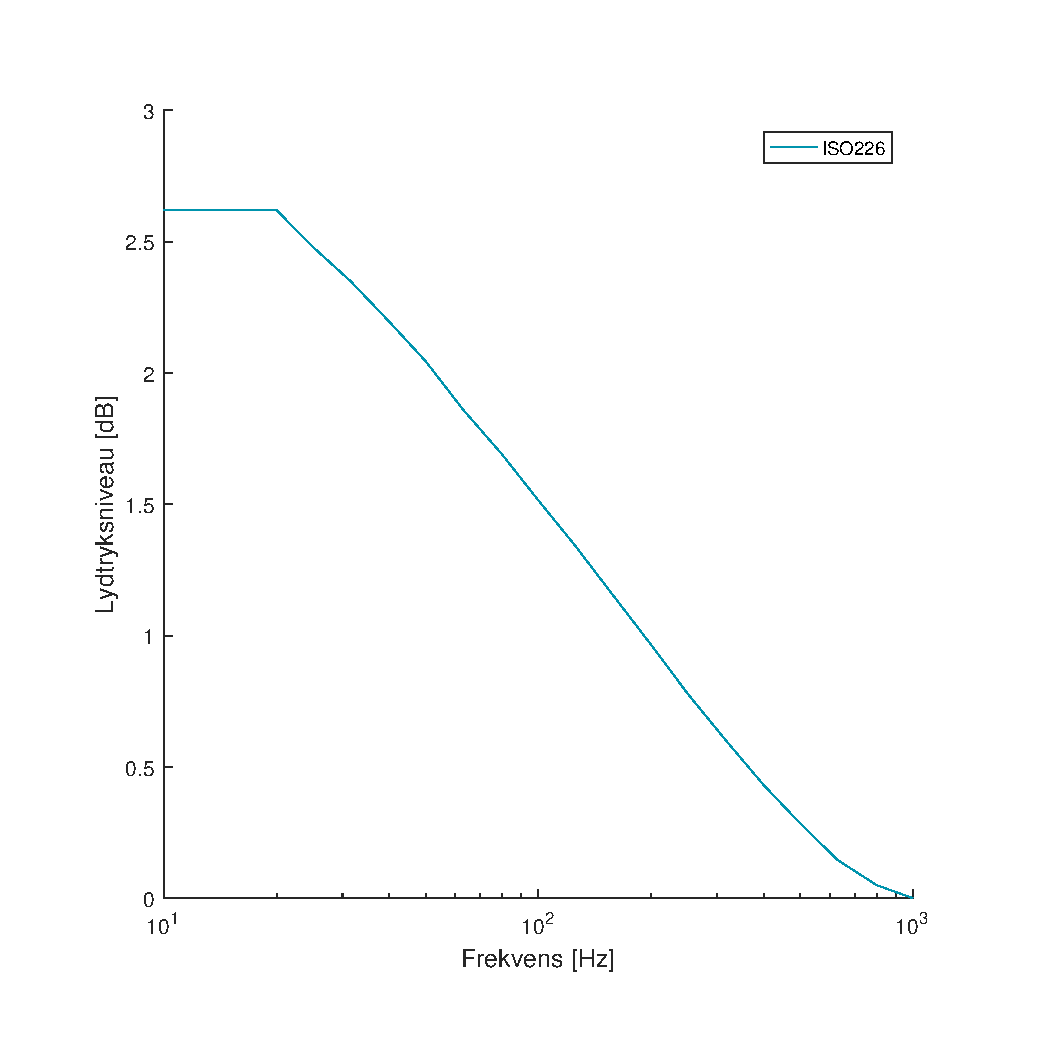
\includegraphics[resolution=300,scale=0.7]{Figure/DesignAfFilter/IdeelFilterRespons}
	\caption{Ideel filterrespons på 2.62dB/1.699dekade for det mindst forstærkende filter, i forhold til ISO226.} 
	\label{fig:IdeelFilterRespons}
\end{figure}
\noindent
%
Tilsvarende skal der også være filtre, der skal dæmpe frekvenser på 20Hz med 2.62dB for hver 5dB der skrues op i forhold til referencens lydtryksniveau. Dæmpningen skal aftage lineært mod 1000Hz, hvorefter der ikke længere skal dæmpes. Dæmpningen skal være 2.62dB over 1.699dekade for det mindst dæmpende filter.

Den maksimale forstækning med et referencelydtryksniveau på 80dB er 20.96dB ved et lydtryksniveau på 40dB. Forstærkningen skal være 20.96dB over 1.699dekade for det mest forstærkende filter. Den maksimale dæmpning når referencens lydtryksniveau er på 80dB er 10.48dB, ved 100dB. Dæmpningen skal derfor være 10.48dB over 1.699dekade for det mest dæmpende filter\\ 

\subsection{Krav til styresystem}
\label{Systemkrav_Styresystem}
%
Da styresystemet består af flere moduler, fokuseres på ét modul ad gangen. Rækkefølgen vil være bestemt baseret på signalets vej fra filtrene igennem styresystemet, hvorfor der først fokuseres på multiplekserne og dernæst på stereovolumenkontrollen.\\
\blankline	
\textbf{Multiplekser}\\
Multiplekserne skal kunne modtage to forskellige analoge spændinger på indgangsterminalerne og levere én af de to spændinger på udgangsterminalen, på baggrund af et digitalt binært input. På den måde virker multiplekserne som en kontakt, der kan vælge at sende én af to inputs videre som output. Kontaktfunktionen skal virke mellem hvert af de enten forstærkende eller dæmpende filtre. Derudover skal én kontaktfunktion anvendes til at vælge mellem rækken af enten forstærkende eller dæmpende filtre. I alt skal der bruges én kontakt for hvert forstærkende filter i systemet, plus én kontakt til at vælge mellem rækken af enten forstærkende eller dæmpende filtre.\\         
\blankline
%
\textbf{Stereovolumenkontrol}\\
Stereovolumenkontrollen anvendes så udviklingen af lydtryksniveauet perciperes lineært. Endvidere er det nødvendigt, at volumenkontrollens gain afdækker hele det dB-spektrum, der arbejdes indenfor. dB-spektrummet der arbejdes indenfor ligger mellem 40dB og 100dB, hvorfor stereovolumenkontrollen skal have et gain på 60dB. Stereovolumenkontrollen skal kunne modtage en analog spænding på indgangsterminalen og levere et logaritmisk justeret output på udgangsterminalen.\\
\blankline 
%
\textbf{A/D konverter}\\
A/D konverteren har til formål at give multiplekserens kontakt besked om at skifte position ud fra en analog spænding. A/D konverteren skal derfor kunne modtage en analog spænding på indgangsterminalen og levere et digital binært output på udgangsterminalerne, svarende til spændingen på indgangsterminalen. 
\blankline
%
\textbf{Komparator}\\
Komparatoren har til formål at vurdere om lydtryksniveauet er over eller under referencens lydtryksniveau. Outputtet sendes videre til multiplekseren, hvis kontakt skifter position og vælger mellem rækken af filtre der enten forstærker eller dæmper. Komparatoren skal kunne modtage en positiv eller negativ spænding på den ikke-inverterende indgangsterminal og afgøre om spændingen er over eller under referencespændingen på den inverterende indgangsterminal. Komparatoren skal på udgangsterminalen levere et digitalt højt output hvis indgangsterminalens spænding er over referencens og et digitalt lavt output hvis indgangsterminalens spænding er under referencens.   
\blankline
%
\textbf{Dobbeltensretter}\\
Dobbeltensretteren har til formål at levere et analogt signal, der kun kan være positivt. Den modtager signalet fra differensforstærkeren og sender det videre til A/D konverteren. Dobbeltensretteren skal kunne modtage både et positivt eller negativt signal på indgangsterminalen og leverer den numeriske værdi af amplitudens spænding på udgangsterminalen. 
\blankline 	
%
\textbf{Differensforstærker}\\
Differensforstærkeren har til formål at afgøre hvor langt der skrues væk fra referencens lydtryksniveau. Dette gøres ved at udregne differencen mellem de spændinger, som den modtager på de to indgangsterminaler, der kommer fra volumenpotentiometeret og referencepotentiometeret. Differensforstærkeren skal kunne modtage en spænding på hver af de to indgangsterminaler og levere differencen mellem spændingerne på udgangsterminalen.   
\blankline	
%
\subsection{Krav til brugergrænseflade}
\label{Krav_Brugergraenseflade}
%
Da brugergrænsefladen består af flere moduler og funktioner, vil der fokuseres på ét modul ad gangen. Først fokuseres der på brugergrænsefladens forside, derefter displayet og slutteligt brugergrænsefladens bagside. \\
\blankline	
\textbf{Volumenkontrol}\\
Brugeren af produktet skal have mulighed for at ændre volumen. Volumenændring skal udelukkende tilgås via ét enkelt potentiometer. Det skal ved hjælp af volumenpotentiometeret være muligt at skrue ned til 40dB, ligesom det skal være muligt via volumenpotentiometeret at skrue op til 100dB.  
\blankline  	
\textbf{Referencekontrol}\\
Brugeren af produktet skal have mulighed for at ændre reference. Referencekontrollen skal udelukkende tilgås via ét enkelt potentiometer. Det skal ved hjælp af referencepotentiometeret være muligt at ændre referencen $\pm$5dB, i forhold til den fastlagte reference på 80dB. Referencen skal derfor kunne ændres til 75dB og 85dB.   
\blankline	
\textbf{Display}\\
Brugeren af produktet skal have mulighed for at følge med i, hvilke filtre der aktuelt anvendes. Displayet skal give visuel feedback til brugeren. Ved ændring af filtre skal den visuelle feedback fremgå på displayet i realtid da forsinket feedback kan forvirre brugeren. Det skal være muligt at frakoble displayet så brugeren ikke længere får visuel information om hvilke filtre der aktuelt anvendes. Ydermere anvendes displayet for at fejlfinde på systemet, for på den måde at undgå at de forkerte filtre aktiveres.         
\blankline		
\textbf{Bypass}\\
Brugeren af produktet skal have mulighed for at bypasse filtrene. Bypass betyder at signalet ikke filtreres men i stedet ledes uden om filtrene.   
%
\subsection{Krav til eksterne grænseflader}
\label{EksterneGraenseflader}
%
Udover de tre overordnede modul grupperinger, forefindes der to nødvendige og essentielle eksterne grænseflader; forsyningsspænding og lyd.\\
\blankline	
\textbf{Forsyningsspænding}\\
Den positive forsyningsspænding skal være +8V. Spændingen skal kunne leveres via bananstik.\\
Den negative forsyningsspænding skal være -5V. Spændingen skal kunne leveres via bananstik.\\
Jord (DGND og AGND) skal være 0V. Spænding skal kunne leveres via samme bananstik.\\ 
\blankline 
\textbf{Lyd}\\
Inputsignalet skal være analogt. Systemet er designes til kun at skulle behandle analoge signaler.\\ 
Inputtet leveres via Jack 3.5mm. Derved er det let at tilslutte systemet til en computer eller mobiltelefon, da disse ofte har et Jack på 3.5mm.\\
Outputtet, som stadig skal være analogt, leveres via RCA plug. Derved er det let at tilslutte systemet til en forstærker, da disse ofte har en RCA plug.\\
%
\section{Opsummering af specifikke systemkrav}
\label{OpsummeringAfSpecifikkeSystemkrav}
% Filtre
\textbf{1. Filtre:}\\
§1.1 Filtrene kan dæmpe eller forstærke frekvenser på 20Hz med 2.62dB for hver 5dB der skrues op eller ned i forhold til referencens lydtryksniveau. Dæmpningen eller forstærkningen sker lineært mod 1000Hz, hvorefter der ikke længere dæmpes eller forstærkes.\\
§1.2 Filterets forstærkningen er 2.62dB over 1.699dekade for det mindst forstærkende filter.\\ 
§1.3 Filterets forstærkningen er 20.96dB over 1.699dekade for det mest forstærkende filter.\\ 
§1.4 Filterets dæmpningen er 2.62dB over 1.699dekade for det mindst dæmpende filter.\\
§1.5 Filterets dæmpningen er 10.48dB over 1.699dekade for det mest dæmpende filter.\\ 
\blankline 
% Styresystem
\textbf{2. Styresystem:}\\
§2.1 Multipleksernes kontakter skal kunne modtage to forskellige analoge spændinger på indgangsterminalerne og levere én af de to spændinger på udgangsterminalen på baggrund af et digitalt binært input.\\
%
§2.2 Stereovolumenkontrollen skal kunne modtage en analog spænding på indgangsterminalen og levere et logaritmisk justeret output på udgangsterminalen.\\
%
§2.3 A/D konverteren kan modtage en analog spænding på indgangsterminalen og levere et digitalt binært output på udgangsterminalerne svarende til spændingen på indgangsterminalen.\\ 
%
§2.4 Komparatoren skal på udgangsterminalen levere et digitalt højt output hvis indgangsterminalens spænding er over referencen og et digitalt lavt output hvis indgangsterminalens spændingen er under referencen.\\
%
§2.5 Dobbeltensretteren kan modtage en positiv eller negativ spænding på indgangsterminalen og levere den numeriske værdi af amplitudens spænding på udgangsterminalen.\\
%
§2.6 Differensforstærkeren kan modtage en spænding på hver af de to indgangsterminaler og levere differencen mellem spændingerne på udgangsterminalen.\\
%
\blankline 
% Brugergrænseflade 
\textbf{3. Brugergrænseflade:}\\
§3.1 Volumenkontrollen kan med et potentiometer vælges til at være mellem 40dB og 100dB.\\ 
%
§3.2 Referencespændingen kan med et potentiometer ændres $\pm$5dB i forhold til 80dB.\\
%
§3.3 Displayet kan visuelt repræsentere ændringer af filtre i realtid.\\ 
%
§3.4 Bypass kan lede signalet udenom filtrene.\\
%
§3.5 Forsyningsspændingen leveres via bananstik med et potentiale på henholdsvis +8V, -5V og GND.\\ 
\blankline	
% ekstern grænseflade 
\textbf{4. Ekstern grænseflade:}\\
§4.1 Lydsignalet leveres analogt\\ 
§4.2 Lydinputtet leveres via RCA plug.\\
§4.3 Lydoutputtet leveres via Jack 3.5mm.\\
